\section{Methodlogy}

\subsection{Study Area}
This study is based on data from 13 countries across five continents: Australia, Brazil, China, Costa Rica, Ecuador, Italy, Mexico, New Zealand, Norway, Pakistan, South Africa, Taiwan, and Vietnam. The selection of these nations was guided by two primary criteria: a significant diversity of soil types , as indexed by the Harmonized World Soil Database (HWSD) and a high frequency of recorded landslides between 2006 and 2017, as documented in NASA's Global Landslide Catalog.
\begin{figure}[htbp]
    \centerline{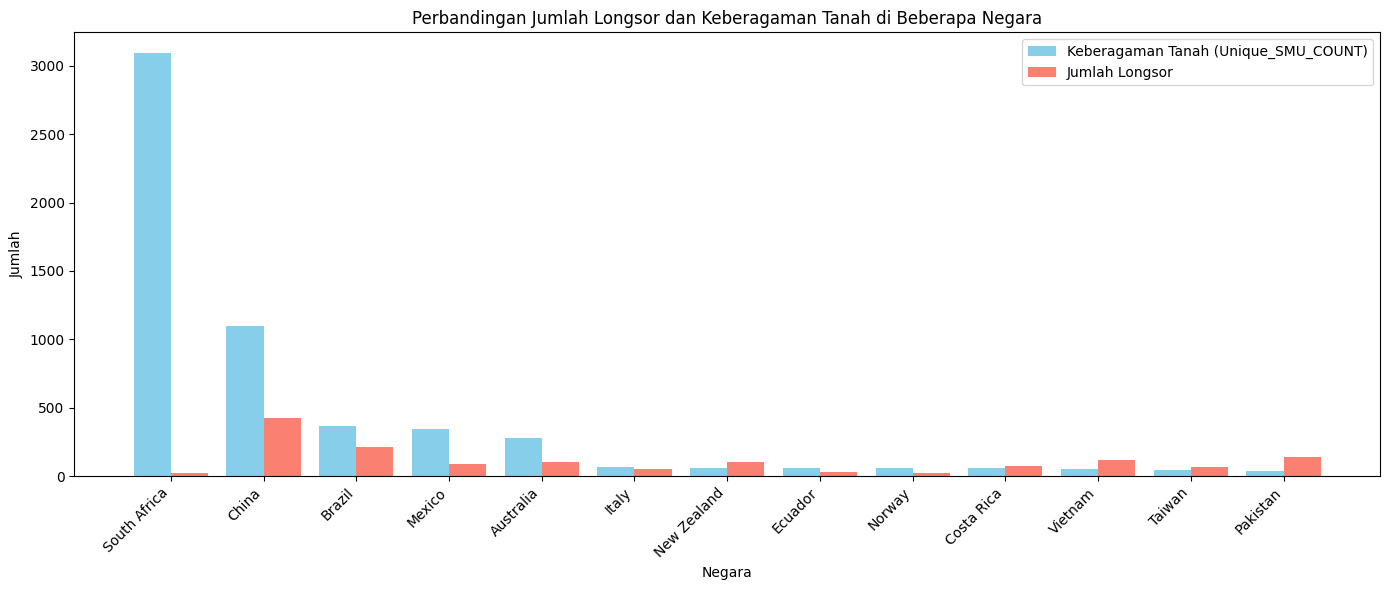
\includegraphics[width=\linewidth]{fig1.png}}
    \caption{Landslide events vs. unique soil characteristics.}
    \label{fig:landslide-soil-distribution}
\end{figure}
Figure~\ref{fig:landslide-soil-distribution} illustrates the distribution of landslide events and soil diversity (represented by the count of unique Soil Mapping Units) for the selected countries. For most nations, a general correspondence is observed between the two metrics. South Africa, however, presents a notable exception, exhibiting exceptionally high soil diversity relative to its number of recorded landslides. This broad geographical scope inherently introduces significant variations in other key landslide-triggering factors, such as climate patterns (ranging from tropical to temperate), topography (from steep mountainous terrain to gentle hills), and land cover, which is essential for developing a globally generalizable model.


\subsection{Datasets}
This study integrates data from three primary sources. Soil characteristics were derived from the Harmonized World Soil Database (HWSD), a 30 arc-second raster database providing presents soil information collected from various regional and national sources, including the European Digital Map (ESDE), the 1:1,000,000 scale Soil Map of China, and various legacy soil maps from FAO. Data from these different sources were harmonized using standard procedures. The database consists of a raster image that is linked to the attribute database through a unique code of the soil mapping unit. For each mapping unit, the database provides information on the composition of the soil types present in it (dominant soils and accompanying soils). It also contains quantitative data on soil physical and chemical properties for two depth layers, namely topsoil (0-30 cm) and subsoil (30-100 cm). These attributes include organic carbon content, pH, water holding capacity, soil depth, cation exchange capacity, clay fraction, salinity, and soil texture. Table 1 describes the classification of data sources and their data types and table 2 describes general information on the soil mapping unit composition.

\begin{table}[H]
\caption{Data Sources and Outputs in the Harmonized World Soil Database}
\centering
\begin{tabular}{|c|l|l|l|} % Only 4 columns, not 5
\hline
\textbf{No.} & \multicolumn{1}{|c|}{\textbf{Data Source}} & \multicolumn{1}{|c|}{\textbf{Format}} & \multicolumn{1}{|c|}{\textbf{Output}} \\
\cline{2-4} % Line only under columns 2 to 4
\textbf{} & \textbf{\textit{Database Name}} & \textbf{\textit{Data Type}} & \textbf{\textit{Resolution/Quantity}} \\
\hline
1 & ESDB & Geo. DB & Raster $\sim$1 km \\
\hline
2 & Soil Map China & Digital Map & Raster $\sim$1 km \\
\hline
3 & SOTER (SOTWIS) & Soil & Raster $\sim$1 km \\
\hline
4 & Soil Map World & Digital Map & Raster $\sim$1 km \\
\hline
5 & Soil Profile DB & Profile Data & 9607 profiles \\
\hline
\multicolumn{4}{l}{$^{\mathrm{a}}$ESDB: European Soil Database. Geo. DB: Geographic Database.} \\
\multicolumn{4}{l}{$^{\mathrm{b}}$Soil Map of China; SOTER: World Soils and Terrain Database.} \\
\multicolumn{4}{l}{$^{\mathrm{c}}$Soil Profile DB: Soil Profile Database.} \\
\multicolumn{4}{l}{$^{\mathrm{d}}$Input Scale/Resolution for raster data (1:1M or 1:10M).} \\
\multicolumn{4}{l}{$^{\mathrm{e}}$Input Scale/Resolution for SOTER databases (1:2.5M – 5M).}
\end{tabular}
\label{tab:hwsd_sources_compact}
\end{table}

Historical landslide event data were obtained from the NASA Global Landslide Catalog (GLC), from which we extracted all documented rainfall-triggered landslides occurring between 2006 and 2017. Finally, all data were geographically contextualized using the Natural Earth “Admin 0 – Countries” vector dataset (1:10m scale) to define the national administrative boundaries for the study area.


\subsection{Method}

The methodology adopted in this study is systematically illustrated in Figure~\ref{fig:research-workflow}. The research commenced with an extensive literature review on soil characteristics and landslide occurrences to gather relevant data. Subsequently, three distinct datasets were compiled and integrated.

\begin{figure}[htbp]
    \centerline{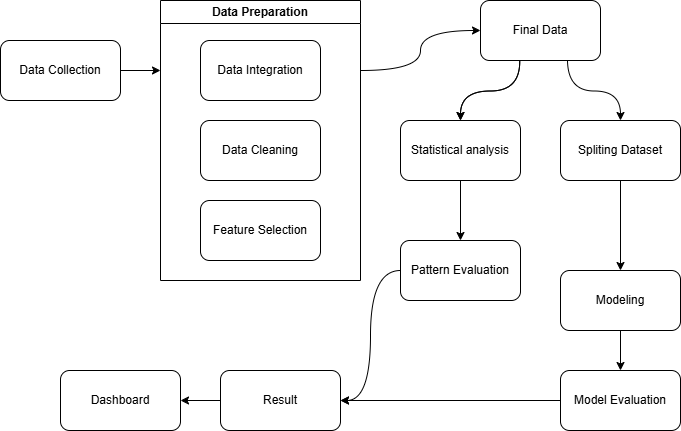
\includegraphics[width=\linewidth]{fig2.png}}
    \caption{research workflow}
    \label{fig:research-workflow}
\end{figure}
This integration process was guided by two primary references: the HWSD Technical Report and Instructions and a technical note by D.G. Rossiter, Processing the Harmonized World Soil Database (Version 1.2) in R. A detailed flowchart of the data integration procedure is presented in Figure~\ref{fig:data-integration-workflow}. From the study area, a total of 2,210 landslide and non-landslide data, each corresponding to different soil characteristics, were identified.

\begin{table}[H]
\caption{Field Availability in Soil Databases (Simplified)}
\centering
\begin{tabular}{|p{2cm}|p{2.8cm}|c|}
\hline
\textbf{Field} & \textbf{Description} & \textbf{DSMW} \\
\hline
\multicolumn{3}{|l|}{\textbf{General}} \\
\hline
ID & Database ID & $\surd$ \\
MU\_GLOBAL & Global Unit ID & $\surd$ \\
COVERAGE & Coverage & $\surd$ \\
ISSOIL & Soil indicator & $\surd$ \\
SHARE & Share in Unit & $\surd$ \\
SU\_SYMBOL & Symbol & $\surd$ \\
\hline
\multicolumn{3}{|l|}{\textbf{Phases and Additional}} \\
\hline
PHASE1 & Phase 1 & $\surd$ \\
ROOTS & Root obstacles &  \\
AWC\_CLASS & AWC Class & $\surd$ \\
\hline
\end{tabular}
\label{tab:soil_field_availability_small}
\end{table}

\begin{figure}[htbp]
    \centerline{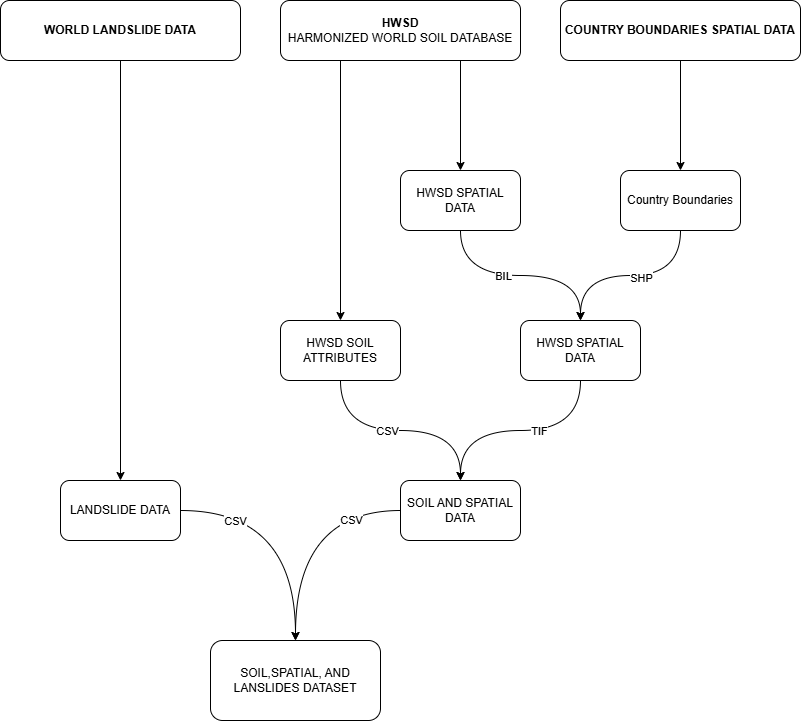
\includegraphics[width=\linewidth]{fig3.png}}
    \caption{Data Integration Workflow}
    \label{fig:data-integration-workflow}
\end{figure}

Following data integration, a comprehensive data preprocessing phase was conducted. This began with data cleaning, in which missing values were imputed using the median of their respective columns. Subsequently, outlier handling was performed using the Interquartile Range (IQR) method\cite{mthd01}. This analysis revealed numerous outliers across most feature columns; these were also imputed using the column-specific median in order to maintain data integrity.
The next stage focused on feature selection. Features were removed based on three criteria: identifier columns (as listed in Table~\ref{tab:soil_field_availability_small}), columns containing only a single unique value, and those with low feature importance scores method. A machine learning-based approach using the XGBoost algorithm was employed to assess the importance of each remaining feature\cite{mthd02}. The results of this analysis, visualized in Figure~\ref{fig:feature-importance}, identified two features—\texttt{AWC\_CLASS} and \texttt{S\_CASO4}—with an importance score of zero. Consequently, these non-contributory features were removed from the dataset.

The final preprocessing step was data transformation. Label encoding was applied to the categorical feature 'COUNTRY'. This method was selected for its suitability with tree-based models, which are invariant to the ordinal relationships that might be artificially introduced by other encoding techniques\cite{mthd03}. 
\begin{figure}[htbp]
    \centerline{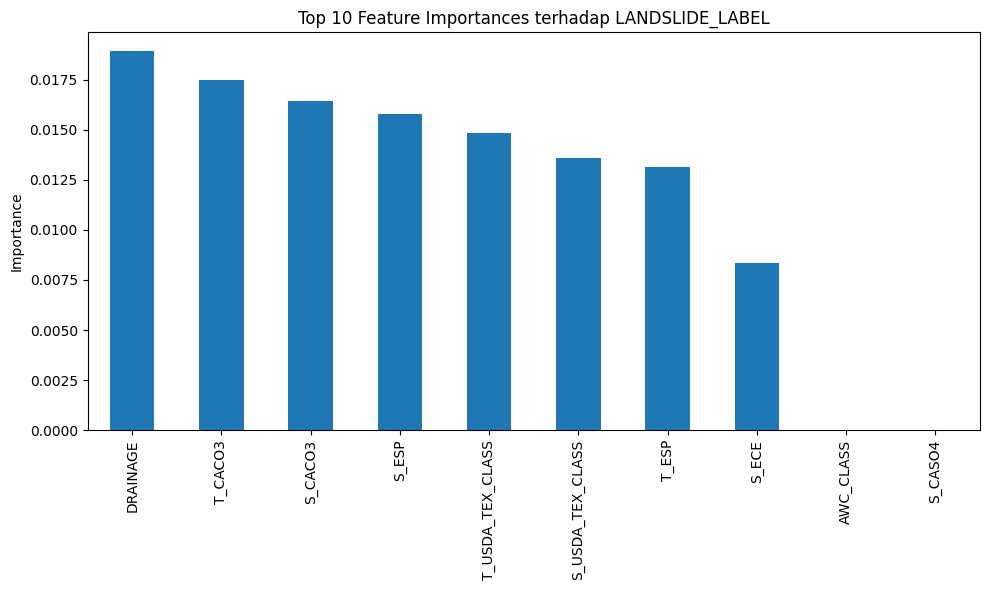
\includegraphics[width=\linewidth]{fig4.png}}
    \caption{Feature Importance Analysis}
    \label{fig:feature-importance}
\end{figure}
This study employs two primary analytical approaches: statistical analysis and machine learning modeling.

\subsubsection{statistical analysis}
Statistical analysis was conducted to identify significant differences in soil characteristics between two predefined groups: locations where landslides occurred (labeled as 1) and locations where they did not (labeled as 0). To achieve this, both parametric and non-parametric hypothesis tests were applied, specifically the independent samples t-test and the Mann-Whitney U test\cite{mthd04}.

The main objective of these tests was to calculate the p-value for each soil feature. The p-value quantifies the probability that an observed difference between the groups is merely due to random chance. A lower p-value indicates a more statistically significant difference, suggesting that the corresponding soil feature is a meaningful differentiator between landslide and non-landslide conditions.

The mathematical formulation for the independent samples t-test is presented in Equation~\ref{eq:t_test}, while the formula for the Mann-Whitney U test is detailed in Equation~\ref{eq:mann_whitney}.

\begin{equation} \label{eq:t_test}
t = \frac{\bar{x}_1 - \bar{x}_2}{s_p \cdot \sqrt{\frac{1}{n_1} + \frac{1}{n_2}}}
\end{equation}
where $s_p$ is the pooled standard deviation, calculated as:
\begin{equation} \label{eq:sp_pooled}
s_p = \sqrt{\frac{(n_1 - 1)s_1^2 + (n_2 - 1)s_2^2}{n_1 + n_2 - 2}}
\end{equation}

For the Mann-Whitney U test, the U statistic is given by:
\begin{equation} \label{eq:mann_whitney}
U = \min(U_1, U_2)
\end{equation}
where:
\begin{align}
U_1 &= n_1n_2 + \frac{n_1(n_1 + 1)}{2} - R_1 \label{eq:U1} \\
U_2 &= n_1n_2 + \frac{n_2(n_2 + 1)}{2} - R_2 \label{eq:U2}
\end{align}
\subsubsection{machine learning modeling}
For the primary classification task, this study utilized the Extreme Gradient Boosting (XGBoost) model\cite{mthd05}. XGBoost is a highly efficient and scalable implementation of the gradient tree boosting algorithm, widely regarded as a state-of-the-art machine learning method. It employs a regularized boosting technique, which effectively mitigates overfitting and thereby enhances model accuracy and generalization performance. The selection of XGBoost was motivated by its numerous advantages, including its scalability across diverse scenarios, inherent capability to handle sparse data, low computational resource requirements, high-performance speed, and ease of implementation. The fundamental principle of the boosting algorithm is to sequentially combine the outputs of multiple weak learners---in this case, Classification and Regression Trees (CARTs)---to create a single, robust predictive model. The core of the algorithm aims to minimize the regularized objective function, as formulated in Equation~\ref{eq:objective_function}. This function is composed of two main parts: a loss function and a regularization term. The loss function measures the discrepancy between the actual target ($y_i$) and the prediction ($\hat{y}_i$). The second component, the regularization term detailed in Equation~\ref{eq:regularization_term}, penalizes the complexity of the model to avoid overfitting. The overall algorithmic process is described by Equations~\ref{eq:objective_function} through \ref{eq:simplified_objective_function_t}.
% Equation (3) - Objective Function
\begin{equation} \label{eq:objective_function}
L(\Phi) = \sum_i l(\hat{y}_i, y_i) + \sum_k \Omega(f_k)
\end{equation}

% Equation (4) - Regularization Term
\begin{equation} \label{eq:regularization_term}
\Omega(f) = \gamma T + \frac{1}{2} \lambda \|w\|^2
\end{equation}
where:
\begin{itemize}
    \item $T$: the number of leaves in the tree;
    \item $w$: the score of each leaf;
    \item $\gamma, \lambda$: the regularization degrees.
\end{itemize}

% Equation (5) - Objective Function at iteration t
\begin{equation} \label{eq:objective_function_t}
L^{(t)}(\Phi) = \sum_{i=1}^n l(y_i, \hat{y}_i^{(t-1)} + f_t(x_i)) + \Omega(f_t)
\end{equation}

In order to speed up the optimization process, second order Taylor expansion is applied to the objective. After removing the constant terms, a simplified objective function at step $t$ is given in Equation~\ref{eq:simplified_objective_function_t}.

% Equation (6) - Simplified Objective Function at iteration t
\begin{equation} \label{eq:simplified_objective_function_t}
\tilde{L}^{(t)} = \sum_{i=1}^n \left[ g_i f_t(x_i) + \frac{1}{2} h_i f_t^2(x_i) \right] + \Omega(f_t)
\end{equation}
where:
\begin{align} \label{eq:g_h_definitions}
g_i &= \partial_{\hat{y}_i^{(t-1)}} l(y_i, \hat{y}_i^{(t-1)}) \\
h_i &= \partial_{\hat{y}_i^{(t-1)}}^2 l(y_i, \hat{y}_i^{(t-1)})
\end{align}
The preprocessed dataset was partitioned for training and validation using a 5-fold StratifiedKFold cross-validation scheme\cite{mthd06}. This approach effectively splits the data into an 80\% training set and a 20\% testing set during each fold, while critically preserving the original class distribution (landslide vs. non-landslide) across all folds. This stratification is essential for ensuring reliable model evaluation on an imbalanced dataset. To address the class imbalance issue, the SMOTE (Synthetic Minority Over-sampling Technique) was applied to the training data to synthetically oversample the minority (landslide) class\cite{mthd07}.

The XGBoost classification algorithm was used and evaluated in this study. To enhance the models' sensitivity to the positive class (landslide), a class weight adjustment mechanism was integrated into the training process. Hyperparameter optimization was conducted efficiently using Bayesian Optimization implemented via BayesSearchCV\cite{mthd08}, facilitating an effective search for the optimal parameter combination within a predefined search space.

Model performance was assessed using a suite of standard classification metrics. The Confusion Matrix served as the foundation for performance analysis\cite{mthd09}, categorizing predictions into four distinct outcomes: True Positives (TP), False Positives (FP), True Negatives (TN), and False Negatives (FN), as illustrated in Figure 5.

The primary evaluation metric for this study was the F1-Score, which is the harmonic mean of precision and recall, providing a balanced measure of performance on imbalanced data. Furthermore, the classification threshold was tuned to achieve a desired level of recall. The Receiver Operating Characteristic (ROC) curve was also utilized to visualize the discriminative ability of the models across various thresholds. This curve is generated by plotting the True Positive Rate (TPR) against the False Positive Rate (FPR), where the area under the curve (AUC-ROC) provides an aggregate measure of performance across all classification thresholds.
\begin{figure}[H]
    \centerline{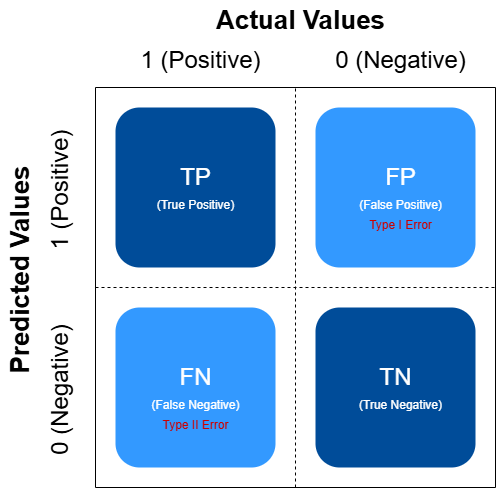
\includegraphics[width=\linewidth]{fig5.png}}
    \caption{Metrics for evaluating classification performance.}
    \label{fig}
\end{figure}

The sensitivity (True positive or Recall) tells the proportion of positive class (landslides locations) that are correctly classified as landslides Equation~\ref{eq:sensitivity}. In contrast, the specificity (True Negative Rate) tells the proportion of negative class (non-landslides locations) that are correctly classified as non-landslides Equation~\ref{eq:specificity}. Between sensitivity and specificity lies False Negative Rate (FNR), which signifies the proportion of landslide points wrongly classified as landslides Equation~\ref{eq:FNR}. The False Positive Rate (FPR) tells the proportion of non-landslides incorrectly classified as non-landslides Equation~\ref{eq:FPR}.

\begin{equation} \label{eq:sensitivity}
\text{sensitivity} = \frac{TP}{TP + FN}
\end{equation}

\begin{equation} \label{eq:specificity}
\text{specificity} = \frac{TN}{TN + FP}
\end{equation}

\begin{equation} \label{eq:FNR}
\text{FNR} = \frac{FN}{TP + FN}
\end{equation}

\begin{equation} \label{eq:FPR}
\text{FPR} = \frac{FP}{TN + FP} = 1 - \text{specificity}
\end{equation}




